%=======================================================================
%  LABORATORIO N.o 4 - DIODOS LIMITADORES Y SUJETADORES
%  Curso : Circuitos Electronicos  (2026-2)
%  UCSP  - Facultad de Ingenieria - Ing. Electronica y de Telecomunicaciones
%  Docente     : Ebert San Roman Castillo
%  Laboratorio : Ing. Jeanpier Ancori Sanchez
%
%  Version 1 - Transcripcion de la guia del docente
%    "Lab. 02 - v2026-1 - Diodos limitadores, sujetadores y rectificadores.doc"
%  (copia en ../Originales) al formato de los laboratorios 1 a 3: mismo
%  preambulo, misma cabecera, mismo encabezado/pie y numeracion en romanos.
%
%  Por decision del autor solo se trabaja el FORMATO. No se anaden notas
%  tecnicas, cajas de seguridad, ejemplos ni contenido propio. Sobre el
%  original solo se hizo:
%    - Corregir erratas evidentes: "1n4007" -> "1N4007", "10uf" -> 10 uF,
%      "1KHz" -> 1 kHz, "como se genero" -> "como se genero" con tilde,
%      "AC(alternator)" -> "AC (alternator)".
%    - Dejar que LaTeX numere secciones, figuras y apartados.
%    - Reemplazar la portada escaneada ("2 Experiencia - Diodos rectificadores")
%      por la cabecera que construye este archivo.
%    - Las figuras 1, 2 y 5 venian en el .doc como EMF; se rasterizan a PNG
%      a 4x. Las demas son los PNG embebidos, sin retocar.
%    - Las tablas "Figura / Comentario" del original se dibujan con
%      \cuadrorespuesta, con espacio para pegar la captura y comentar.
%
%  Version 2 - Correcciones de fondo, una por una, para la Analog Discovery
%  Studio.
%    1. Medida del puente (V.2, paso ii). W1 tiene un borne en la masa de la
%       tarjeta y la carga del puente no: si el extremo inferior de R se une a
%       GND se cortocircuita un diodo y se ve media onda. Los canales del
%       osciloscopio son diferenciales por el conector MTE, asi que la carga se
%       mide con 1+/1- y la fuente con 2+ en W1 y 2- en GND. La figura 5 decia
%       220 Vrms / 60 Hz y el texto pide 5 V de pico a 1 kHz: se rerotula la
%       fuente (5Vpk, 1kHz). La captura sin tocar queda en
%       rectificador_con_capacitor_original.png.
%       Las figuras 2 y 5 conservan su simbolo de masa en el negativo del
%       puente: el simulador lo necesita. La advertencia va solo en el texto.
%    2. Sujetador de la figura 7 (V.4). Con W1 (+-5 V) no se llega a los 15 V
%       de pico de la figura, y con 5 V y la bateria de 10 V el diodo no
%       conduce nunca: salida igual a entrada. La bateria pasa a ser la fuente
%       V- de la tarjeta a -2 V en el anodo, y la salida queda entre -2,7 y
%       +7,3 V. Figura rerotulada (5 V, -5 V, 2 kHz, 2 V, "kOhm" en minuscula)
%       y marcado el borne + del electrolitico, que va hacia el diodo. El
%       simbolo del capacitor se deja como en el libro, por decision del
%       autor: el "+" va sobre la placa del lado del diodo.
%    3. Polaridad del electrolitico tambien en el diseno de la figura 8: la
%       salida queda por debajo de la entrada, el + va hacia la entrada. Y se
%       avisa de que con 100 kOhm cada diodo cae menos de 0,7 V.
%    4. Filtro del puente (V.2): 10 y 200 uF con 1 kOhm a 1 kHz dan 0,18 V y
%       9 mV de rizado, indistinguibles en pantalla, y los picos de carga del
%       de 200 uF piden a W1 una corriente que su hoja de datos no garantiza.
%       Pasan a 2,2 uF (~0,8 V) y 10 uF (~0,18 V). El paso i arma la figura 2
%       y el iii agrega el capacitor, como en la figura 5.
%    5. Materiales: el generador y el osciloscopio son la tarjeta; fuera el
%       ceramico de 100 nF y la de 10 kOhm, que no se usaban; entra la de
%       100 kOhm; cantidades segun la figura 6 (cinco diodos, cuatro de 1 k).
%    6. Formato del curso, como el Laboratorio 3: objetivos que cubren
%       recortadores y sujetadores, "Conocimientos previos" sin "uso de
%       equipos", titulos sin puntaje, cuestionario de 3 preguntas y
%       conclusiones 5 cualitativas + 5 cuantitativas. Las figuras 3 y 4 son
%       del Boylestad: atribucion en nota al pie y fuera el "FIG. 2.100" que
%       traia pegado la figura 4. En la figura 6 las fuentes pasan de
%       10Vrms / 1Hz a 5Vpk / 1kHz, y V.3 dice que fuente de la tarjeta
%       sustituye a cada bateria (en esa figura V8 y V4 van invertidas).
%
%  Version 3 - Por indicacion del docente salen los rectificadores de media
%  onda y de onda completa: ya se trabajan en el Laboratorio 3 (fuente DC).
%    - Fuera sus subsecciones en "Conocimientos previos" y en "Desarrollo", con
%      las figuras que los acompanaban. Con ellas desaparecen las correcciones
%      1 y 4 de la version 2. rectificador_media_onda.png,
%      rectificador_onda_completa.png y rectificador_con_capacitor*.png quedan
%      en imagenes/ pero ya no se usan.
%    - El titulo pasa a "Diodos limitadores y sujetadores" (cabecera, pie y
%      metadatos del PDF).
%    - Objetivos y contenido teorico sin rectificadores. Los materiales pierden
%      el electrolitico de 10 uF, que era solo del filtro.
%    - Cuestionario: las preguntas 1 y 2 eran del rectificador. Pasan a ser una
%      del nivel de recorte (por que 2,7 V y no 2 V) y otra de la condicion
%      5RC >> T/2 en el sujetador (con R = 100 ohm, 5RC = 1,1 ms frente a
%      T/2 = 0,25 ms: la salida ya se inclina).
%
%  Version 4 - Por indicacion del autor se incorporan los ejercicios 3 a 7 de
%  la guia del docente "Lab. 03 - v2026-1 - Diodos zener.docx" (copia en
%  ../Originales). Quedan como V.3 a V.7, despues de los sujetadores:
%    - V.3 regulador con RV2 (image16 -> zener_regulador_rv.png)
%    - V.4 Vi fijo, RL variable (image11 -> zener_rl_variable.png)
%    - V.5 Vi variable, RL fijo (image12 -> zener_vi_variable.png)
%    - V.6 diodo clipper (image8 -> zener_clipper.png)
%    - V.7 investigacion
%  Se transcriben tal cual, sin puntaje en el titulo (formato del curso) y
%  solo con erratas evidentes corregidas: V.6 remitia a la "figura 5", que es
%  la de V.4, y ahora apunta a su propia figura; "regula" -> "regule",
%  "Evalue" -> "Evalue" con tilde. Las figuras de V.4 y V.5 son del Boylestad:
%  atribucion en nota al pie. Entran el objetivo y el tema del Zener como
%  regulador (del mismo original) y los materiales que piden los ejercicios.
%  PENDIENTES por revisar con el autor, sin tocar todavia:
%    - V.3 da IZM = 10 mA e IZK = 25 mA: la corriente minima mayor que la maxima.
%    - V.3 alimenta con 14 V; la tarjeta da como mucho 5 V programables o el
%      rail fijo de +12 V.
%    - V.4 y V.5 trabajan con 12 a 16 V: solo se pueden analizar y simular.
%    - V.6 no dice que Zener usar: se listan dos 1N4730A (3,9 V), los unicos
%      que recortan con los 5 V de pico de W1.
%
%  Version 5 - Se ordena la practica, sin anadir notas (pedido del autor).
%    - Materiales: una sola lista ordenada por tipo (diodos, resistencias,
%      potenciometros, capacitores y montaje) con lo que piden todos los
%      ejercicios. Del original del Zener entran el cable telefonico solido y
%      los alicates, en lugar de "cablecillos".
%    - Conocimientos previos: entra IV.3, la teoria del Zener del original
%      (image9 -> zener_regulador_sin_carga.png, image13 -> zener_curva.png).
%      Asi las dos familias del desarrollo tienen su teoria delante.
%    - Desarrollo: primero el diodo de silicio (limitadores, sujetadores y el
%      diseno del sujetador, que era el paso iii y pasa a apartado propio);
%      despues el Zener, de lo que se calcula a lo que se monta: Vi fijo y RL
%      variable, Vi variable y RL fijo, regulador con RV2 y clipper.
%    - La investigacion sale del desarrollo y va al informe final: no se hace
%      en el laboratorio.
%
%  Version 6 - Cambio de planes: sale todo el Zener (lo de las versiones 4 y 5).
%    - Fuera el objetivo, el tema del contenido teorico, IV.3 (teoria del
%      Zener), los cuatro apartados del desarrollo (Vi fijo y RL variable, Vi
%      variable y RL fijo, regulador con RV2 y clipper) y la investigacion del
%      informe final. Con ellos desaparecen los PENDIENTES de la version 4.
%      Las imagenes zener_*.png quedan en imagenes/ pero ya no se usan.
%    - Materiales: solo lo que piden limitadores, sujetador y diseno. Fuera los
%      Zener 1N4740A y 1N4730A, la resistencia de 10 kOhm a 0,5 W y los
%      potenciometros de 1 y 5 kOhm, que eran de los ejercicios del Zener.
%      Sale tambien el cable telefonico solido (pedido del autor).
%    - Cantidades: los circuitos se arman de uno en uno y se reutilizan las
%      piezas (la tarjeta solo tiene dos canales). Ya no se cuenta como en la
%      version 2, sumando la figura entera. Lo maximo que pide un circuito:
%      2 diodos (recortador de D2 y D5, y el diseno: 1,35 V son dos diodos de
%      silicio en serie), 1 resistencia de 1 kOhm (cada recortador), 1 de
%      100 kOhm y 1 electrolitico de 2,2 uF (sujetador y diseno). Se piden
%      3 diodos y no 2: uno de repuesto (pedido del autor). Se agregan
%      "resistencias de otros valores conocidos" (pedido del autor). Tambien
%      con repuesto: 2 resistencias de cada valor y 2 electroliticos. Entran
%      los jumpers macho-macho, en lugar del cable telefonico.
%=======================================================================

\documentclass[11pt,a4paper]{article}

%------------------------------------------------------------- idioma
% Compilar con XeLaTeX (no con pdflatex): Trebuchet MS es una fuente TrueType
% del sistema y solo fontspec, bajo XeLaTeX o LuaLaTeX, sabe cargarla.
\usepackage{fontspec}
\setmainfont{Trebuchet MS}[
  Path            = C:/Windows/Fonts/,
  Extension       = .ttf,
  UprightFont     = trebuc,
  BoldFont        = trebucbd,
  ItalicFont      = trebucit,
  BoldItalicFont  = trebucbi,
  Ligatures       = TeX
]
\usepackage[spanish,es-nodecimaldot]{babel}
\usepackage{microtype}

%----------------------------------------------------------- geometria
\usepackage[left=2.4cm,right=2.4cm,top=3.1cm,bottom=2.6cm,headheight=30pt,
            footskip=1.2cm]{geometry}

%------------------------------------------------------------ graficos
\usepackage{graphicx}
\usepackage{xcolor}
\usepackage{float}
\usepackage{placeins}
\usepackage[font=small,labelfont=bf,labelsep=period]{caption}
\usepackage{subcaption}
\graphicspath{{imagenes/}}

%-------------------------------------------------------------- tablas
\usepackage{array}
\usepackage{tabularx}
\usepackage{multirow}

%----------------------------------------------------- matematicas / SI
\usepackage{amsmath,amssymb}
\usepackage{siunitx}
\sisetup{
  output-decimal-marker = {,},
  per-mode              = symbol,
  mode                  = match,
  detect-weight         = true,
  detect-family         = true
}

%--------------------------------------------------------------- listas
\usepackage{enumitem}
\setlist[itemize]{itemsep=3pt,topsep=4pt,parsep=0pt}
\setlist[enumerate]{itemsep=8pt,topsep=4pt,parsep=0pt}

%------------------------------------------------------------ comandos
\usepackage{pgffor}

% Lineas punteadas para respuestas del alumno: \lineasresp{n}
% Con 11 pt entre renglones (el valor del Laboratorio 3) sobraban tres
% renglones de las conclusiones en una novena pagina; con 8 pt cabe en ocho.
\newcommand{\lineasresp}[1]{%
  \par\vspace{6pt}%
  \foreach \i in {1,...,#1}{\noindent\rule{\linewidth}{0.4pt}\par\vspace{8pt}}%
}

% Recuadro "Figura / Comentario" del original: una celda alta para pegar la
% captura del osciloscopio y otra debajo para el comentario.
\newcommand{\cuadrorespuesta}{%
  \par\vspace{6pt}\noindent
  \begin{tabularx}{\linewidth}{|>{\centering\arraybackslash}X|}
    \hline
    \rule{0pt}{4.4cm}\raisebox{2.1cm}{\textcolor{black!45}{Figura}}\\
    \hline
    \rule{0pt}{2.0cm}\raisebox{0.9cm}{\textcolor{black!45}{Comentario}}\\
    \hline
  \end{tabularx}\par\vspace{8pt}%
}

%----------------------------------------------------- compaginacion
\usepackage{needspace}
\usepackage{etoolbox}
\pretocmd{\section}{\needspace{5\baselineskip}}{}{}
\pretocmd{\subsection}{\needspace{4\baselineskip}}{}{}
\widowpenalty=10000
\clubpenalty=10000

%---------------------------------------------------- encabezado / pie
\usepackage{fancyhdr}
\pagestyle{fancy}
\fancyhf{}
\fancyhead[L]{\footnotesize UCSP --- Facultad de Ingeniería\\
              Ing. Electrónica y de Telecomunicaciones}
\fancyhead[R]{\footnotesize 2026-2 Circuitos Electrónicos\\
              Ebert San Román Castillo}
\fancyfoot[L]{\footnotesize Laboratorio N.\textsuperscript{o} 4 --- Diodos limitadores y sujetadores}
\fancyfoot[R]{\footnotesize Página \thepage\ de \pageref{LastPage}}
\renewcommand{\headrulewidth}{0.4pt}
\renewcommand{\footrulewidth}{0.4pt}
\usepackage{lastpage}

%------------------------------------------------------- numeracion
\renewcommand{\thesection}{\Roman{section}}
\renewcommand{\thesubsection}{\arabic{subsection}}
\renewcommand{\thesubsubsection}{\thesubsection.\arabic{subsubsection}}
\setcounter{secnumdepth}{3}

%-------------------------------------------------------- hiperenlaces
\usepackage[hidelinks,pdfusetitle]{hyperref}
\usepackage{xurl}
\hypersetup{
  pdftitle={Laboratorio 4 - Diodos limitadores y sujetadores},
  pdfsubject={Circuitos Electronicos - Guia de practicas},
  pdfauthor={Ebert San Roman Castillo; Jeanpier Ancori Sanchez},
  pdfkeywords={electronica, diodo, recortadores, limitadores, sujetadores,
               1N4007, Analog Discovery Studio, Proteus, Multisim, osciloscopio}
}

% babel-spanish rotula las tablas como "Cuadro"; los originales dicen "Tabla".
\addto\captionsspanish{\renewcommand{\tablename}{Tabla}}

\begin{document}

%=======================================================================
%  CABECERA DE LA GUIA
%=======================================================================
\begin{center}
    {\normalsize\bfseries PRIMERA UNIDAD: DIODOS Y APLICACIONES BÁSICAS}
\end{center}

\vspace{0.55cm}

% Cabecera identica a la de los laboratorios 1 a 3.
\begingroup
\renewcommand{\tabularxcolumn}[1]{m{#1}}
\renewcommand{\arraystretch}{2.0}
\setlength{\tabcolsep}{12pt}
\noindent
\begin{tabularx}{\textwidth}{|>{\centering\arraybackslash}m{2.2cm}|>{\centering\arraybackslash}X|>{\centering\arraybackslash}m{3.0cm}|}
\hline
\rule{0pt}{2.1cm}{\fontsize{58}{58}\selectfont\bfseries 4}
    & \begin{minipage}[c]{\linewidth}\centering
          {\large\bfseries Guía de Prácticas}\\[7pt]
          {\Large\bfseries Diodos Limitadores\\ y Sujetadores}
      \end{minipage}
    & {\Large\bfseries Nota}\\
\hline
\multicolumn{3}{|l|}{\rule{0pt}{1.3cm}\large\textbf{Grupo:}~\rule{4.6cm}{0.4pt}%
    \hfill\large\textbf{Fecha:}~\rule{4.6cm}{0.4pt}\hspace{2mm}}\\
\hline
\multicolumn{3}{|l|}{\rule{0pt}{1.2cm}\large\textbf{Alumno(s):}~\rule{11.2cm}{0.4pt}\hspace{2mm}}\\
\multicolumn{3}{|l|}{\rule{0pt}{1.2cm}\phantom{\large\textbf{Alumno(s):}}~\rule{11.2cm}{0.4pt}\hspace{2mm}}\\
\hline
\end{tabularx}
\endgroup

\vspace{0.8cm}

%=======================================================================
\section{Objetivos}
%=======================================================================
\begin{itemize}
    \item Familiarizar al estudiante con el comportamiento del diodo rectificador de
          silicio en AC.
    \item Medir con el osciloscopio las señales de entrada y de salida de circuitos
          recortadores y sujetadores.
    \item Analizar cómo los circuitos recortadores limitan la señal de entrada y cómo los
          sujetadores desplazan su nivel DC.
    \item Diseñar un circuito sujetador a partir de la forma de onda de salida requerida.
\end{itemize}

%=======================================================================
\section{Contenido teórico}
%=======================================================================
\begin{itemize}
    \item Análisis de circuitos con diodos, modelos de circuito equivalente para el diodo
          y análisis rápido de circuitos con diodos.
    \item Circuitos limitadores y sujetadores.
\end{itemize}

%=======================================================================
\section{Equipos y materiales}
%=======================================================================
\noindent\textbf{Laboratorio:} Electrónica de Comunicaciones.

\vspace{0.25cm}
\noindent\textbf{Equipos y dispositivos:}
\begin{itemize}
    \item Tarjeta Analog Discovery Studio: generador de funciones \texttt{W1}, osciloscopio
          de dos canales y fuentes \texttt{V+} y \texttt{V-}.
\end{itemize}

\noindent\textbf{Software:}
\begin{itemize}
    \item Simulador Multisim o Proteus.
\end{itemize}

\vspace{0.25cm}
% Sin el Zener la lista es mas corta y el titulo quedaba solo al pie de la
% primera pagina: se exige sitio para el titulo y los primeros elementos.
\needspace{6\baselineskip}
\noindent\textbf{Materiales y fungibles} (deben ser adquiridos por los alumnos):
\begin{itemize}
    % --- Diodos
    \item 03 diodos rectificadores de silicio 1N4001, 1N4002 o 1N4007.
    % --- Resistencias
    \item 02 resistencias de \qty{1}{\kilo\ohm}.
    \item 02 resistencias de \qty{100}{\kilo\ohm}.
    \item Resistencias de otros valores conocidos.
    % --- Capacitores
    \item 02 capacitores electrolíticos de \qty{2.2}{\micro\farad}, de \qty{10}{\volt}
          como mínimo.
    % --- Montaje
    \item Protoboard.
    \item Jumpers macho-macho para protoboard.
    \item Alicates para cortar y pelar alambre.
    \item Multímetro.
    \item Lentes de protección y mandil.
\end{itemize}

\FloatBarrier
%=======================================================================
\section{Conocimientos previos}
%=======================================================================

%-----------------------------------------------------------------------
\subsection{Circuitos recortadores con diodos (clippers)}
%-----------------------------------------------------------------------
Son circuitos que utilizan diodos para recortar o limitar una parte de la señal de entrada
cuando esta supera un determinado nivel de voltaje. De esta forma se evita que la señal
supere ciertos valores positivos o negativos
(figura~\ref{fig:recortadores}).\footnote{Las figuras~\ref{fig:recortadores}
y~\ref{fig:sujetadores} se tomaron de R.~L. Boylestad y L.~Nashelsky,
\emph{Electrónica: teoría de circuitos y dispositivos electrónicos}, capítulo~2.}

% Lado a lado quedaban ilegibles: van a ancho completo, una por pagina,
% con \ContinuedFloat para que ambas sigan siendo la figura 1.
\begin{figure}[H]
  \centering
  \begin{subfigure}[t]{0.85\linewidth}
    \centering
    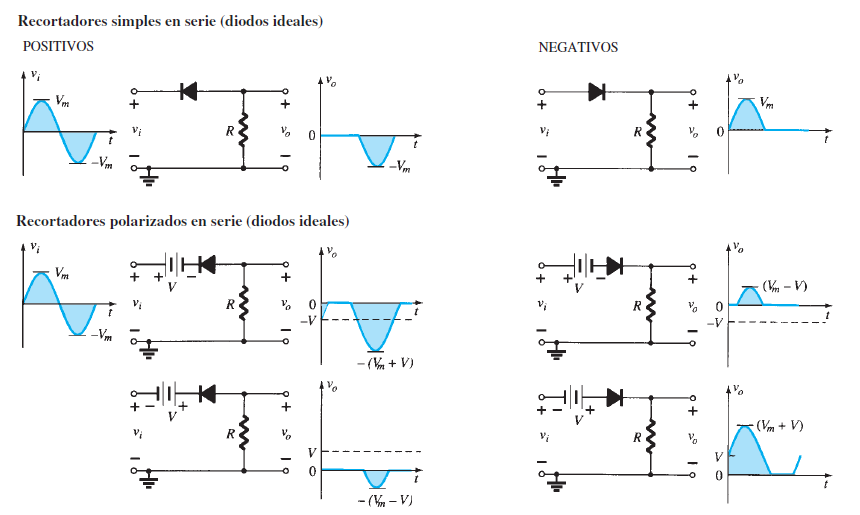
\includegraphics[width=\linewidth]{recortadores_serie.png}
    \caption{Recortadores en serie.}
  \end{subfigure}
  \caption{Circuitos recortadores.}
  \label{fig:recortadores}
\end{figure}

\begin{figure}[H]
  \ContinuedFloat
  \centering
  \begin{subfigure}[t]{0.76\linewidth}
    \centering
    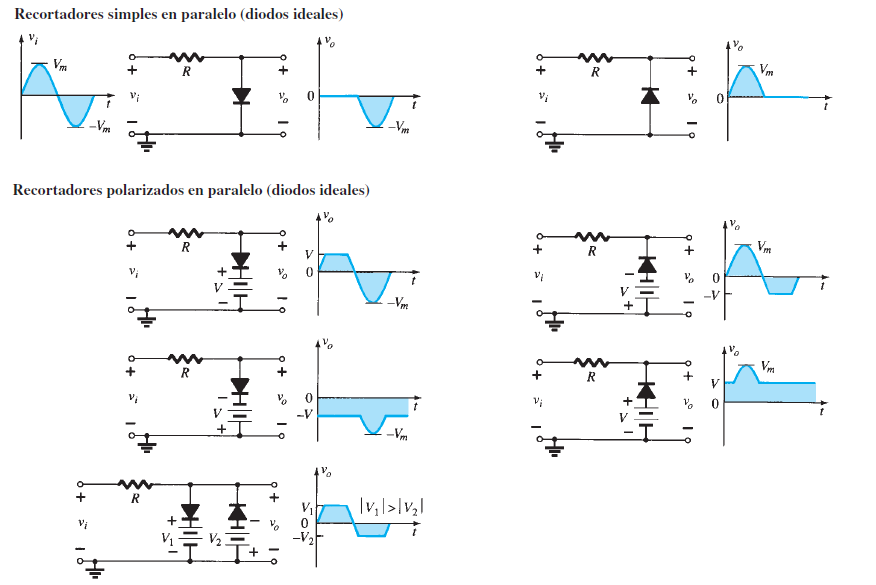
\includegraphics[width=\linewidth]{recortadores_paralelo.png}
    \caption{Recortadores en paralelo.}
  \end{subfigure}
  \caption{Circuitos recortadores (continuación).}
\end{figure}

%-----------------------------------------------------------------------
\subsection{Circuitos sujetadores con diodos (clampers)}
%-----------------------------------------------------------------------
Son circuitos que utilizan diodos, capacitores y resistencias para desplazar el nivel DC de
una señal sin modificar su forma, fijando uno de sus extremos (superior o inferior) a un
nivel de referencia (figura~\ref{fig:sujetadores}). Se debe considerar que
$5\tau=5RC\gg T/2$, de tal manera que el capacitor no se descargue.

\begin{figure}[H]
  \centering
  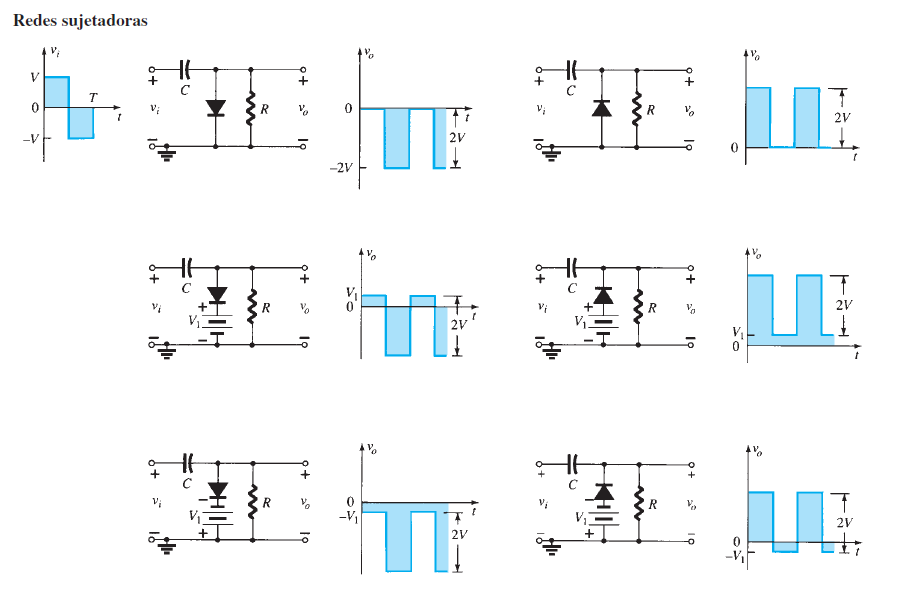
\includegraphics[width=0.8\linewidth]{sujetadores.png}
  \caption{Circuitos sujetadores.}
  \label{fig:sujetadores}
\end{figure}

\FloatBarrier
% El titulo quedaba solo al pie de la pagina: se exige sitio para el titulo,
% la subseccion y los dos primeros pasos.
\needspace{14\baselineskip}
%=======================================================================
\section{Desarrollo del laboratorio}
%=======================================================================

%-----------------------------------------------------------------------
\subsection{Circuitos limitadores}
%-----------------------------------------------------------------------
\begin{enumerate}[label=\roman*., leftmargin=*, labelsep=0.6em]
  \item Construya uno por uno los circuitos de la figura~\ref{fig:circuitos-recortadores}.
        Configure \texttt{W1} como señal sinusoidal de \qty{5}{\volt} pico y
        \qty{1}{\kilo\hertz}. Reemplace las baterías por las fuentes \texttt{V+} y
        \texttt{V-} de la tarjeta, con los valores que indica la figura.
  \item Compare las señales de salida y entrada de cada circuito y comente el resultado.
        Debe indicar cómo se generó la señal de salida.
\end{enumerate}

\begin{figure}[H]
  \centering
  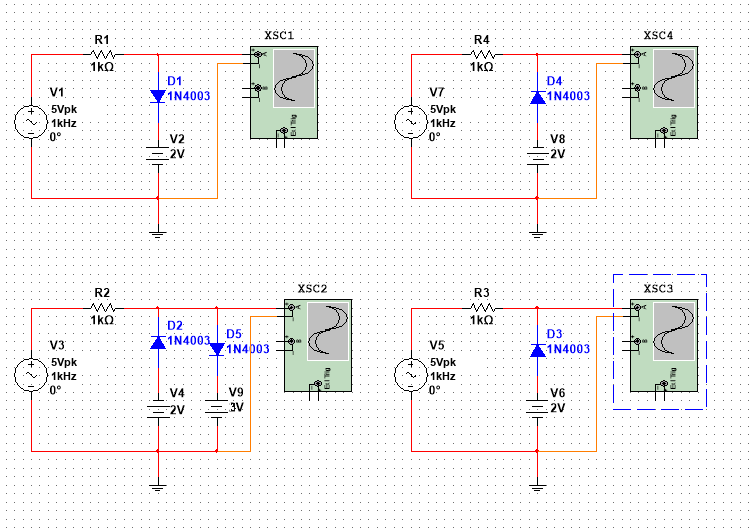
\includegraphics[width=0.78\linewidth]{circuitos_recortadores.png}
  \caption{Circuitos recortadores a implementar.}
  \label{fig:circuitos-recortadores}
\end{figure}

\cuadrorespuesta
\cuadrorespuesta
\cuadrorespuesta
\cuadrorespuesta

%-----------------------------------------------------------------------
\subsection{Sujetadores}
%-----------------------------------------------------------------------
\begin{enumerate}[label=\roman*., leftmargin=*, labelsep=0.6em]
  \item Construya el circuito de la figura~\ref{fig:circuito-sujetador}. Configure
        \texttt{W1} como señal sinusoidal de \qty{5}{\volt} pico y \qty{2}{\kilo\hertz}.
        La batería se sustituye por la fuente \texttt{V-} de la tarjeta ajustada a
        \qty{-2}{\volt}, conectada al ánodo del diodo. El capacitor es electrolítico:
        conecte su terminal positivo hacia la fuente AC y el negativo hacia el cátodo del
        diodo.
  \item Compare la señal de salida con la de entrada y comente el resultado.
        Debe indicar cómo se generó la señal de salida.
\end{enumerate}

\begin{figure}[H]
  \centering
  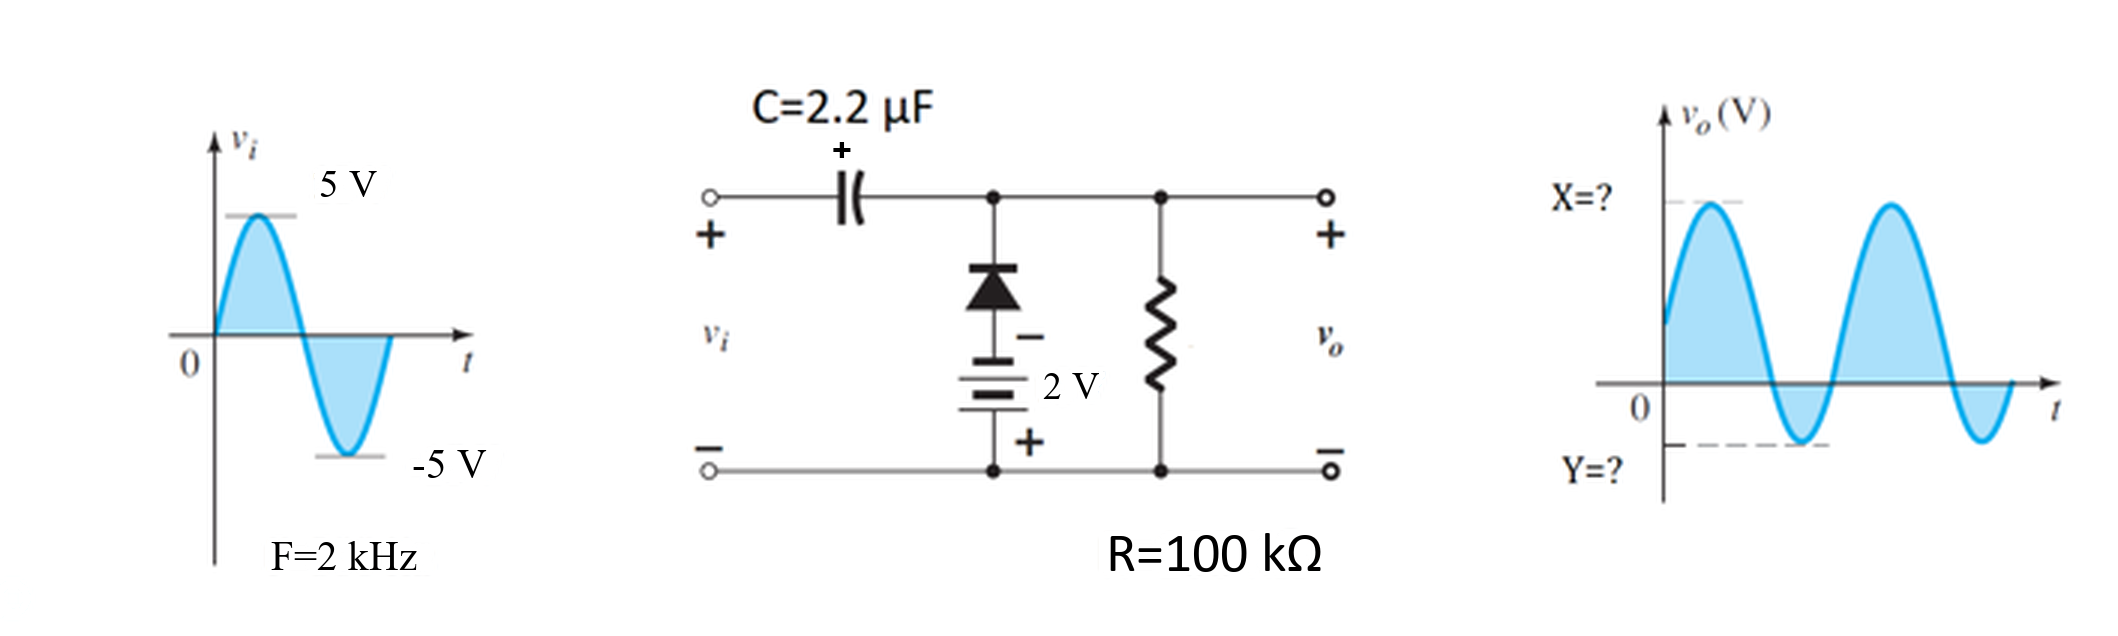
\includegraphics[width=0.78\linewidth]{circuito_sujetador.png}
  \caption{Circuito sujetador.}
  \label{fig:circuito-sujetador}
\end{figure}

\cuadrorespuesta

%-----------------------------------------------------------------------
\subsection{Diseño de un circuito sujetador}
%-----------------------------------------------------------------------
Diseñe un sujetador para que realice la función indicada en la figura~\ref{fig:diseno}.
Configure \texttt{W1} como señal cuadrada de \qty{5}{\volt} pico y
\qty{1}{\kilo\hertz}. Si usa un
capacitor electrolítico, respete su polaridad: en este sujetador la salida queda por debajo
de la entrada, así que su terminal positivo va hacia la entrada. Tenga en cuenta además que
con una resistencia de carga grande cada diodo conduce poca corriente y cae menos de los
\qty{0.7}{\volt} ideales (unos \qtyrange{0.5}{0.55}{\volt}), de modo que el nivel positivo
medido puede quedar por debajo de los \qty{1.35}{\volt} de la figura.

\begin{figure}[H]
  \centering
  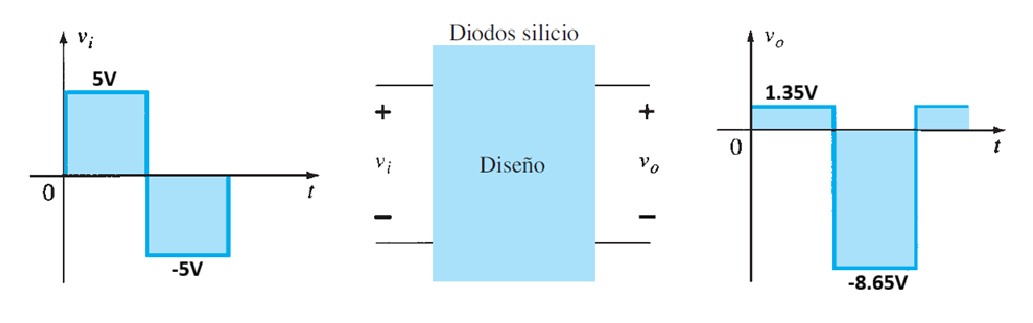
\includegraphics[width=0.65\linewidth]{diseno_sujetador.png}
  \caption{Ejercicio de diseño de circuito sujetador.}
  \label{fig:diseno}
\end{figure}

\cuadrorespuesta

\FloatBarrier
%=======================================================================
\section{Informe final}
%=======================================================================
\begin{enumerate}[label=\textbf{\arabic*.}, leftmargin=*, labelsep=0.6em]
  \item Presente las formas de onda obtenidas en cada punto del desarrollo de la
        práctica, compárelas con lo esperado y analice las diferencias.
\end{enumerate}

\FloatBarrier
%=======================================================================
\section{Cuestionario}
%=======================================================================
\begin{enumerate}[label=\textbf{\arabic*.}, leftmargin=*, labelsep=0.6em]
\item En el recortador de D1 y V2 (figura~\ref{fig:circuitos-recortadores}) la fuente
\texttt{V+} está a \qty{2}{\volt}, pero la salida se recorta cerca de
\qty{2.7}{\volt}. ¿De dónde sale esa diferencia? ¿En qué nivel se recortaría si el diodo
fuera de germanio?
\lineasresp{3}

\item En el sujetador de la figura~\ref{fig:circuito-sujetador}, ¿qué le pasaría a la señal
de salida si la resistencia fuera de \qty{100}{\ohm} en lugar de \qty{100}{\kilo\ohm}?
Justifíquelo con la condición $5RC\gg T/2$.
\lineasresp{3}

\item En el sujetador de la figura~\ref{fig:circuito-sujetador}, ¿qué valores tomarían X e Y
si la fuente \texttt{V-} de \qty{-2}{\volt} se sustituyera por \texttt{V+} a
\qty{2}{\volt}? Justifique su respuesta.
\lineasresp{3}
\end{enumerate}

\FloatBarrier
%=======================================================================
\section{Conclusiones}
%=======================================================================
\begin{itemize}
    \item Redacte como mínimo 05 conclusiones \textbf{cualitativas} y 05
          \textbf{cuantitativas}.
\end{itemize}

\noindent\textbf{Cualitativas}
\lineasresp{10}

\needspace{6\baselineskip}
\noindent\textbf{Cuantitativas}
\lineasresp{10}

\end{document}
